\documentclass{beamer}

\usepackage[T1]{fontenc}
\usepackage[french]{babel}
\usepackage[utf8]{inputenc}

% Choose the Inf theme
\usetheme{Inf}

% Define the title with \title[short title]{long title}
% Short title is optional
\title[Sequoia: A deep root in Linux's filesystem layer]
      {Sequoia: A deep root in Linux's filesystem layer}

%Qualys Security Advisory



% Optional subtitle
\subtitle{CVE-2021-33909}

\date{21 novembre 2024}

% Author information
\author{Duzés Florian}
\institute{\texttt{florian.duzes@u-bordeaux.fr}}

\begin{document}

% Title page
\InfTitlePage

\begin{frame}
  \frametitle{Sommaire}
  \tableofcontents
\end{frame}

\Infsection{Aperçu général}

% Résumé
\frame{
    \frametitle{Résumé}

    Vulnérabilité : size\_t -> int
    \medskip
    \begin{itemize}
        \item Création d'un répertoire avec un chemin > 1Go
        \item Monter ce répertoire dans un espace utilisateur
        \item Suppression dudit répertoire
        \item Écriture d'un chaine de caractère hors limite
        \item Exploitation et accés root        
    \end{itemize}

    Systèmes testés : Ubuntu 20.04, Ubuntu 20.10, Ubuntu 21.04, Debian 11 et Fedora 36  
}

%Historique
\frame{
    \frametitle{Historique}

    \begin{itemize}
        \item Introduite en Juillet 2014
        \begin{itemize}
            \item Linux 3.16 - 058504ed "fs/seq\_file: fallback to vmalloc allocation"
        \end{itemize}
        \item Découverte en Juin 2021
        \item Patch en Juillet 2021
        \begin{itemize}
            \item Correction apporté par : Red Hat Product Security
        \end{itemize}
    \end{itemize}
}

\Infsection{Idée de l'attaque}

% Gestion mémoire des fichiers virtuels
\begin{frame}[fragile]
    \frametitle{Gestion mémoire des fichiers virtuels}
    
    \begin{minted}[breaklines]{c}
    168 ssize_t seq_read_iter(struct kiocb *iocb, struct iov_iter *iter){
 170         struct seq_file *m = iocb->ki_filp->private_data;
 205         /* grab buffer if we didn't have one */
 206         if (!m->buf) {
 207                 m->buf = seq_buf_alloc(m->size = PAGE_SIZE);
 ...
 210         }
 ...
 220         // get a non-empty record in the buffer
 ...
 223         while (1) {
 ...
 227                 err = m->op->show(m, p);
 ...
 236                 if (!seq_has_overflowed(m)) // got it
 237                         goto Fill;
 238                 // need a bigger buffer
 ...
 240                 kvfree(m->buf);
 242                 m->buf = seq_buf_alloc(m->size <<= 1);
 246         }
    \end{minted}
\end{frame}

\begin{frame}[fragile]
    \frametitle{Gestion mémoire des fichiers virtuels}
    
    \begin{minted}[breaklines]{c}
135 static int show_mountinfo(struct seq_file *m, struct vfsmount *mnt)
136 {
...
150                 seq_dentry(m, mnt->mnt_root, " \t\n\\");
    \end{minted}
    \begin{minted}[breaklines]{c}
 523 int seq_dentry(struct seq_file *m, struct dentry *dentry, const char *esc)
 524 {
 525         char *buf;
 526         size_t size = seq_get_buf(m, &buf);
 ...
 529         if (size) {
 530                 char *p = dentry_path(dentry, buf, size);
    \end{minted}
\end{frame}


\begin{frame}[fragile]
    \frametitle{Gestion mémoire des fichiers virtuels}
    \begin{minted}[breaklines]{c}
380 char *dentry_path(struct dentry *dentry, char *buf, int buflen)
381 {
382         char *p = NULL;
...
385         if (d_unlinked(dentry)) {
386                 p = buf + buflen;
387                 if (prepend(&p, &buflen, "//deleted", 10) != 0)
    \end{minted}
    \begin{minted}[breaklines]{c}
 11 static int prepend(char **buffer, int *buflen, const char *str, int namelen)
 12 {
 13         *buflen -= namelen;
 14         if (*buflen < 0)
 15                 return -ENAMETOOLONG;
 16         *buffer -= namelen;
 17         memcpy(*buffer, str, namelen);
    \end{minted}
\end{frame}


\frame{
    \frametitle{Graphique des opérations}
    \begin{center}
        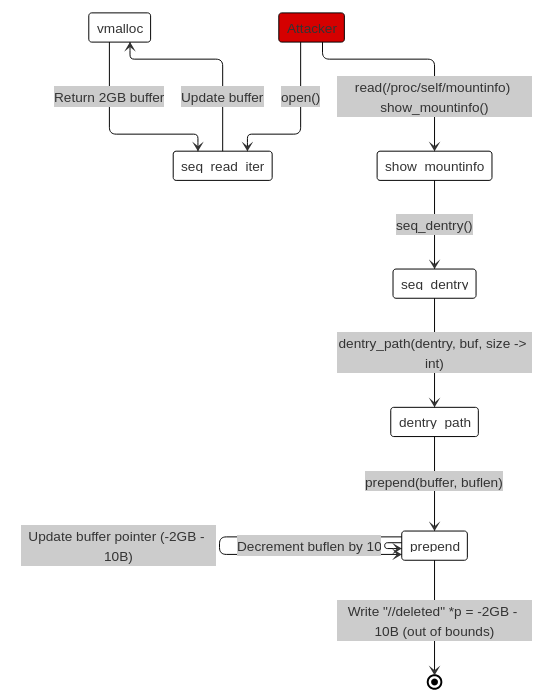
\includegraphics[trim=0cm 0 0cm 0cm, clip, scale = 0.29 ]{graphe.png}    
    \end{center}
}


\frame{
    \frametitle{$\varepsilon$BPF inspiration}
    \begin{center}
        CVE-2020-8835: Linux Kernel Privilege Escalation via Improper eBPF Program Verification    
    \end{center}
}

\Infsection{eBPF - Introduction}

\frame{
    \frametitle{Comment ça marche}
    \begin{center}
        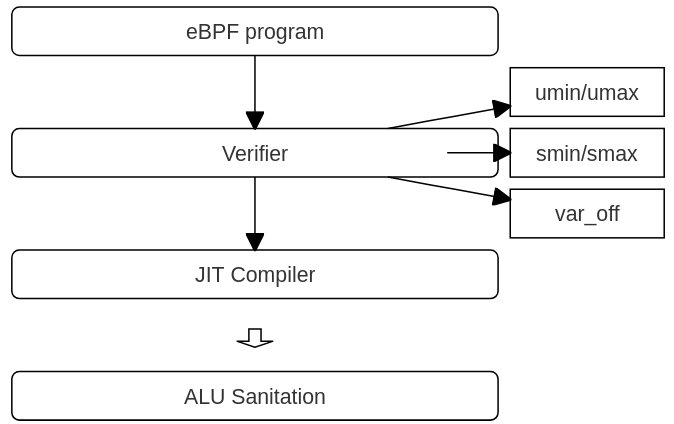
\includegraphics[trim=0cm 0 0cm 0cm, clip, scale = 0.4 ]{eBPF_fonctionnement.png}    
    \end{center}
}
%%%%%%%%%%%%%%%%%%%%%%%%%%%%%%%%%%%%%%%%%%%%%%%%%%%%%
%%                  L'attaque                      %%
%%%%%%%%%%%%%%%%%%%%%%%%%%%%%%%%%%%%%%%%%%%%%%%%%%%%%
\foreach \n in {1, 2, 2a, 2b, 2c, 3, 3a, 3b, 4, 4a, 4b, 5, 6} {
    \begin{frame}
        \frametitle{L'attaque}
        \begin{center}
            \includegraphics[scale=0.38]{eBPF_attack/\n.png}
        \end{center}
    \end{frame}
}

\frame{
    \frametitle{L'attaque}
    \begin{center}
        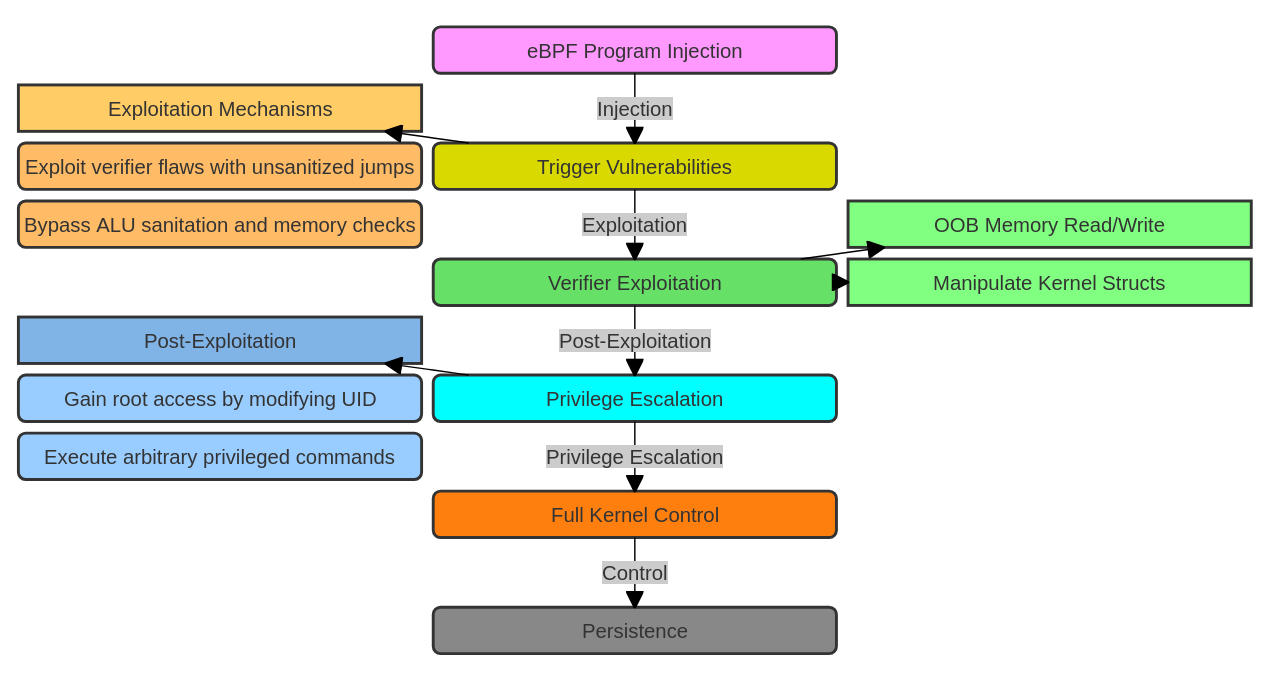
\includegraphics[scale = 0.26]{eBPF_attack/eBPF_attack.png}    
    \end{center}
}


\Infsection{Réunion stratégique}

\frame{
    \frametitle{Point d'accroche - 1}

    \begin{itemize}
        \item \underline{\textbf{Étape 1 : Création et suppression de répertoires}}\\
        \textit{mkdir()} créer une structure de répertoires profondément imbriquée (environ 1 million de répertoires imbriqués), dont la \textbf{longueur totale du chemin dépasse 1 Go}.\\Cette structure est montée via un \textit{bind-mount} dans un espace utilisateur non privilégié, puis supprimée avec \textit{rmdir()}.
    \end{itemize}
}

\frame{
    \frametitle{Point d'accroche - 2}

    \begin{itemize}
        \item \underline{\textbf{Étape 2 : Blocage d'un programme eBPF}}\\
        Un thread est créé pour allouer avec vmalloc() un petit programme eBPF (via l’appel système \textit{BPF\_PROG\_LOAD}).\\Ce thread est ensuite bloqué (via userfaultfd ou FUSE) après que le programme eBPF a été validé par le vérificateur eBPF du noyau, mais avant qu’il ne soit compilé en JIT.
    \end{itemize}
}




\frame{
    \frametitle{Point débordement - 1}

    \begin{itemize}
        \item \underline{\textbf{Étape 3 : Exploitation du dépassement de mémoire}}\\
        Nous ouvrons le fichier /proc/self/mountinfo dans notre espace utilisateur non privilégié. Nous lançons \textit{read()} sur le chemin du répertoire, ce qui provoque l'écriture de la chaîne \textit{//deleted} à un \textbf{décalage de -2 Go - 10 octets} sous le début du tampon alloué par \textit{vmalloc()}.
    \end{itemize}
}

\frame{
    \frametitle{Point débordement - 2}

    \begin{itemize}
        \item \underline{\textbf{Étape 4 : Corruption du programme eBPF}}\\
        La chaîne \textit{//deleted} est utilisée pour \textbf{écraser une instruction du programme eBPF validé}, annulant ainsi les vérifications de sécurité du vérificateur eBPF du noyau.
    \end{itemize}
}


\frame{
    \frametitle{Point exploitation - 1}

    \begin{itemize}
        \item \underline{\textbf{Étape 5 : Arbitrage des lectures/écritures}}\\
        Cette écriture est transformée en lecture/écriture arbitraire de la mémoire du noyau en utilisant les techniques \textbf{btf} et \textbf{map\_push\_elem} décrites par Manfred Paul dans :
        \begin{itemize}
            \item \textit{CVE-2020-8835 - Linux Kernel Privilege Escalation via Improper eBPF Program Verification.}
        \end{itemize}

    \end{itemize}
}

\frame{
    \frametitle{Point exploitation - 2}

    \begin{itemize}
        \item \underline{\textbf{Étape 6 : Escalade de privilèges}}\\
        Nous utilisons cette lecture arbitraire pour localiser le tampon \textbf{modprobe\_path[]} dans la mémoire du noyau. Ensuite, l’écriture arbitraire permet de remplacer son contenu (par défaut \textit{"/sbin/modprobe"}) par un chemin pointant vers notre propre exécutable et ainsi d'obtenir les \textbf{privilèges administrateurs}.

    \end{itemize}
}


\Infsection{Détail de l'attaque}

\begin{frame}
    \frametitle{Répertoire malicieux}

    Il faut un répertoire avec un chemin dépassant 1 Go :
    \begin{itemize}
        \item[->] Théoriquement cela nécessite de créer plus de 4 millions de répertoires imbriqués
        \item[->] En pratique, show\_mountinfo() remplace chaque caractère '{\textbackslash\textbackslash}' dans le chemin par la chaîne de 4 octets "\textbackslash134".
    \end{itemize}    
    Cela réduit à 1 million de répertoires imbriqués la structure nécessaire.
    
\end{frame}

\begin{frame}
    \frametitle{Remplissage de la mémoire ou cartographie du terrain}

    Remplissage des grandes zones libres vmalloc.
    \begin{itemize}
        \item Une partie du chemin très long, créé dans l'étape précédente (étape a), est montée via un bind-mount (MS\_BIND) dans plusieurs espaces utilisateur non privilégiés.
        \item Des tampons sont alloués via des appels read() sur /proc/self/mountinfo (allocation de 768 Mo dans le crsh.c)
    \end{itemize}    
\end{frame}

\begin{frame}[fragile]
    \frametitle{Placement de la charge utile}
    
    Allocations de deux tampons de 1Go et un tampon de 2Go.\\
    Écriture hors-limite.
    \begin{minted}{c}
        "//deleted"
             |
      4KB    v   1GB        4KB        1GB       4KB       2GB
-----|---|---+-------------|---|----------------|---|---------------|
 ... |XXX| seq_file buffer |XXX| seq_file buffer|XXX|seq_file buffer|
-----|---|---+-------------|---|----------------|---|---------------|
         |   |                                      |
         |   \----<----<----<----<----<----<----<---/
         8182B               -2GB-10B
    \end{minted} 
    Calcul de la position de la chaîne : \hfill \textit{\scriptsize{(2*4Ko - 10)}} \\
    $2 * 4Ko = 2 * 4 * 1024 = 8192 $\\$ 8192 - 10 = 8182 $
\end{frame}

\frame{
    \frametitle{Boucher les trous pour faire venir eBPF}
    Allocations via vmalloc() de nombreux messages NETLINK\_USERSOCK.\medskip
    
    
    Objectif, remplir la mémoire de petits objets inutile.
}

\begin{frame}[fragile]
    \frametitle{Construction des petits soldats}

    \begin{enumerate}
        \item Lance 1024 threads -> charge un programme eBPF dans le noyau
        \item Blocage du chargement avant l'allocation en mémoire
    \end{enumerate}
    
    \begin{minted}{c}
2076 static int bpf_prog_load(union bpf_attr *attr, union bpf_attr __user *uattr)
2077 {
....
2100         /* copy eBPF program license from user space */
2101         if (strncpy_from_user(license, u64_to_user_ptr(attr->license),
....
2161         /* plain bpf_prog allocation */
2162         prog = bpf_prog_alloc(bpf_prog_size(attr->insn_cnt), GFP_USER);
    \end{minted} 

\end{frame}


\begin{frame}[fragile]
    \frametitle{Entrée des petits soldats}

    \begin{enumerate}
        \item Libération du premier \textit{seq\_buffer}
        \item Relâche des 1024 threads -> chargement en zone ciblé
    \end{enumerate}
    
    \begin{minted}{c}
      4KB        1GB        4KB        1GB       4KB        2GB
-----|---|-----------------|---|----------------|---|----------------|
 ... |XXX|  eBPF programs  |XXX| seq_file buffer|XXX| seq_file buffer|
-----|---|-----------------|---|----------------|---|----------------|
    \end{minted} 

\end{frame}

\begin{frame}[fragile]
    \frametitle{Choix du héros}

    \begin{itemize}
        \item Blocage d'un thread (ligne 12 795)
        \item[->] Après validation du verifieur eBPF
    \end{itemize}
        \begin{minted}{c}
12640 int bpf_check(struct bpf_prog **prog, union bpf_attr *attr,
12641               union bpf_attr __user *uattr)
12642 {
.....
12795         print_verification_stats(env);
    \end{minted} 
\end{frame}

\begin{frame}[fragile]
    \frametitle{La dame du lac}

    \begin{itemize}
        \item Réécriture d'une instruction eBPF
        \item[->]Esquive des contrôles de sécurité
    \end{itemize}
        \begin{minted}{c}
        "//deleted"
             |
      4KB    v   1GB        4KB        1GB       4KB       2GB
-----|---|---+-------------|---|----------------|---|---------------|
 ... |XXX| seq_file buffer |XXX| seq_file buffer|XXX|seq_file buffer|
-----|---|---+-------------|---|----------------|---|---------------|
         |   |                                      |
         |   \----<----<----<----<----<----<----<---/
         8182B               -2GB-10B
    \end{minted} 
\end{frame}


\begin{frame}
    \frametitle{Assaut final - 1}

    \begin{columns}
        \begin{column}{0.5\textwidth}
        \scriptsize{
            \begin{itemize}
                \item[] BPF\_LD\_IMM64\_RAW(BPF\_REG\_2, BPF\_PSEUDO\_MAP\_VALUE, storage)
                \item[] BPF\_MOV64\_IMM(BPF\_REG\_2, 0)
                \item[] BPF\_LD\_IMM64\_RAW(BPF\_REG\_3, BPF\_PSEUDO\_MAP\_VALUE, control)
                \item[] BPF\_STX\_MEM(BPF\_DW, BPF\_REG\_3, BPF\_REG\_2, 0)
            \end{itemize}
            }
        \end{column}
        \begin{column}{0.5\textwidth}
            \begin{center}
                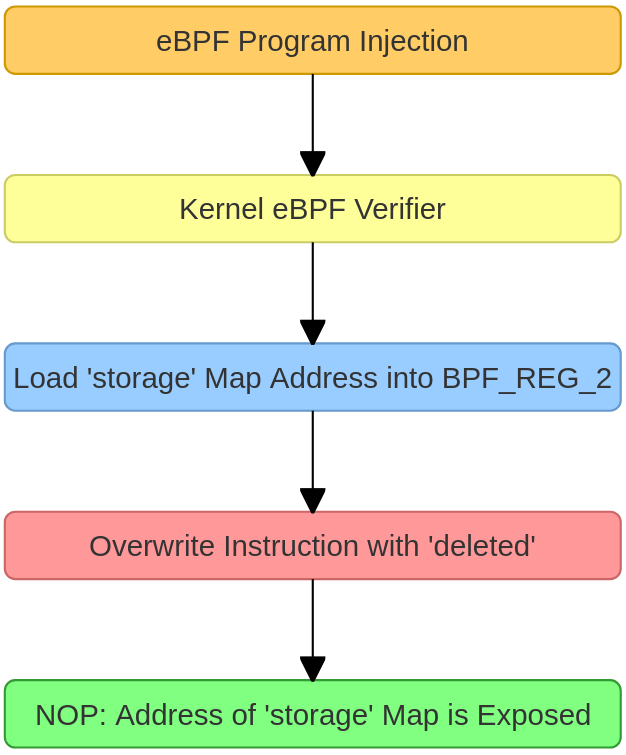
\includegraphics[scale=0.2]{exploit/etape1.png}
            \end{center}
        \end{column}
    \end{columns}
\end{frame}

\begin{frame}
    \frametitle{Assaut final - 2}
    \begin{columns}
        \begin{column}{0.5\textwidth}
        \scriptsize{
            \begin{itemize}
                \item[] BPF\_LD\_IMM64\_RAW(BPF\_REG\_4, BPF\_PSEUDO\_MAP\_VALUE, corrupt)
                \item[] BPF\_ALU64\_IMM(BPF\_ADD, BPF\_REG\_4, 3*64KB/2)
                \item[] BPF\_ALU64\_IMM(BPF\_SUB, BPF\_REG\_4, 3*64KB/4)
                \item[] BPF\_LD\_IMM64\_RAW(BPF\_REG\_3, BPF\_PSEUDO\_MAP\_VALUE, control)
                \item[] BPF\_LDX\_MEM(BPF\_H, BPF\_REG\_7, BPF\_REG\_3, 0)
                \item[] BPF\_ALU64\_REG(BPF\_ADD, BPF\_REG\_4, BPF\_REG\_7)
            \end{itemize}
            }
        \end{column}
        \begin{column}{0.5\textwidth}
            \begin{center}
                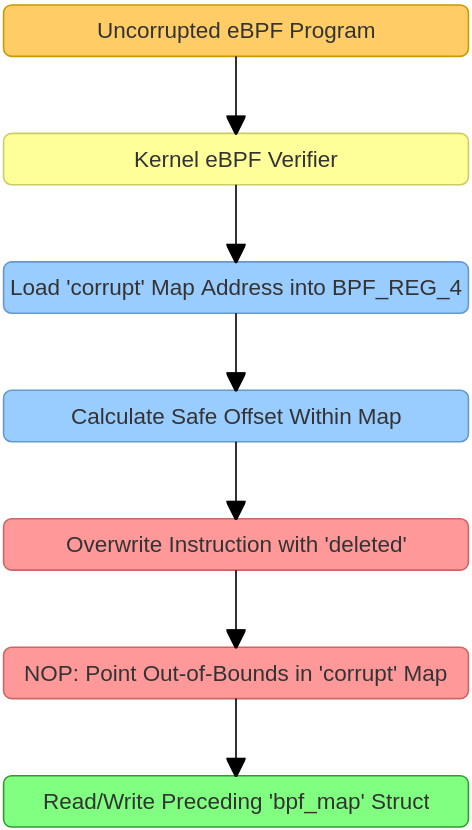
\includegraphics[scale=0.2]{exploit/etape2.png}
            \end{center}
        \end{column}
    \end{columns}
\end{frame}

\begin{frame}
    \frametitle{Assaut final - 3}

        \begin{center}
            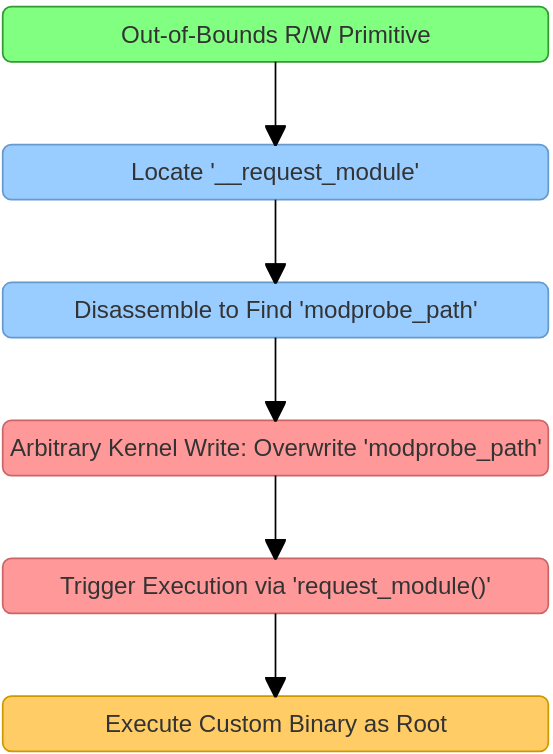
\includegraphics[scale=0.28]{exploit/etape3.png}
        \end{center}

\end{frame}






\Infsection{Solutions}

\frame{
    \frametitle{Contre-mesures}

    Solutions qui permettent de prévenir l'attaque décrite ici : \smallskip

    \begin{itemize}
        \item /proc/sys/kernel/unprivileged\_userns\_clone = 0
        \begin{itemize}
            \item[$+$] Désactiver les espaces de noms utilisateurs non privilégiés
            \item[$-$] L'outil FUSE permet toujours de monter un répertoire long (!)
        \end{itemize}
        \item /proc/sys/kernel/unprivileged\_b = 1
        \begin{itemize}
            \item[$+$] Désactiver eBPF non privilégié
            \item[$-$] on peut cibler d'autres objets (piles de threads)
        \end{itemize}
    \end{itemize}

}

\Infsection{Conclusion}

\begin{frame}
    \frametitle{Sources}
    \begin{enumerate}
        \item https://www.qualys.com/2021/07/20/cve-2021-33909/sequoia-local-privilege-escalation-linux.txt
        \item https://www.thezdi.com/blog/2020/4/8/cve-2020-8835-linux-kernel-privilege-escalation-via-improper-ebpf-program-verification
    \end{enumerate}
\end{frame}

\begin{frame}
    \frametitle{Merci pour votre écoute !}
    \InfContacts
\end{frame}

\end{document}
